\documentclass{standalone}
\usepackage{tikz}
\usetikzlibrary{patterns, positioning}
\usepackage[sfdefault]{ClearSans} %% option 'sfdefault' activates Clear Sans as the default text font
\usepackage[T1]{fontenc}

\begin{document}
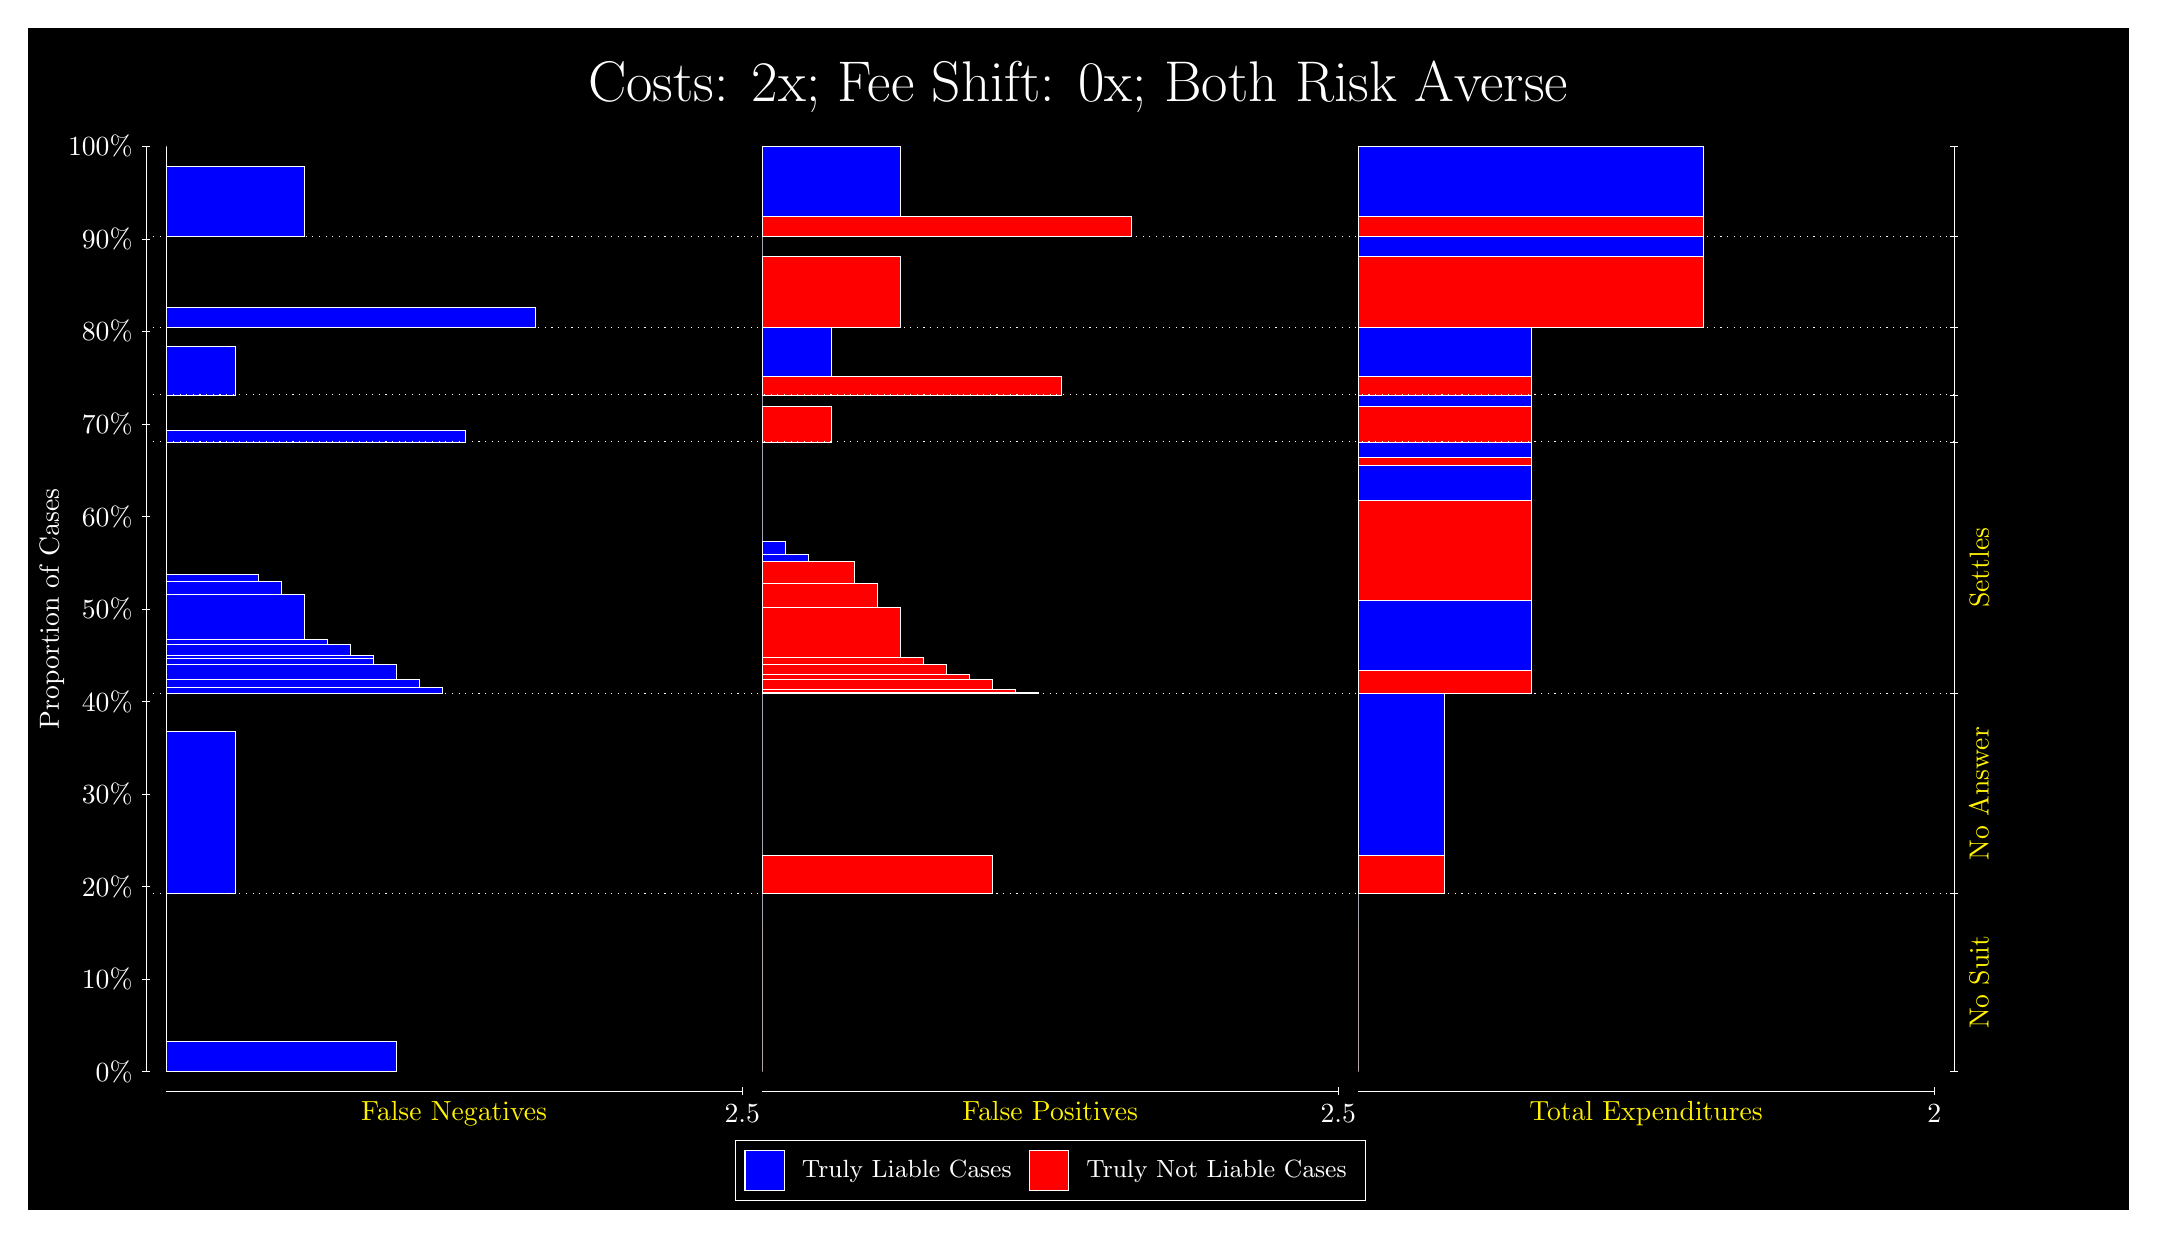
\begin{tikzpicture}
\draw[fill=black] (0,0) rectangle (26.667,15);
\draw[text=white] (0,13.5) rectangle (26.667,15) node[midway] {\huge Costs: 2x; Fee Shift: 0x; Both Risk Averse};
\draw[white, very thin] (1.5,1.75) -- (1.5,13.5);
\node[rotate=90, text=white, anchor=center] at (0.3, 7.625) {Proportion of Cases};
\draw[white, very thin] (1.45,1.75) -- (1.55,1.75);
\node[text=white, anchor=east] at (1.45, 1.75) {0\%};
\draw[white, very thin] (1.45,2.925) -- (1.55,2.925);
\node[text=white, anchor=east] at (1.45, 2.925) {10\%};
\draw[white, very thin] (1.45,4.1) -- (1.55,4.1);
\node[text=white, anchor=east] at (1.45, 4.1) {20\%};
\draw[white, very thin] (1.45,5.275) -- (1.55,5.275);
\node[text=white, anchor=east] at (1.45, 5.275) {30\%};
\draw[white, very thin] (1.45,6.45) -- (1.55,6.45);
\node[text=white, anchor=east] at (1.45, 6.45) {40\%};
\draw[white, very thin] (1.45,7.625) -- (1.55,7.625);
\node[text=white, anchor=east] at (1.45, 7.625) {50\%};
\draw[white, very thin] (1.45,8.8) -- (1.55,8.8);
\node[text=white, anchor=east] at (1.45, 8.8) {60\%};
\draw[white, very thin] (1.45,9.975) -- (1.55,9.975);
\node[text=white, anchor=east] at (1.45, 9.975) {70\%};
\draw[white, very thin] (1.45,11.15) -- (1.55,11.15);
\node[text=white, anchor=east] at (1.45, 11.15) {80\%};
\draw[white, very thin] (1.45,12.325) -- (1.55,12.325);
\node[text=white, anchor=east] at (1.45, 12.325) {90\%};
\draw[white, very thin] (1.45,13.5) -- (1.55,13.5);
\node[text=white, anchor=east] at (1.45, 13.5) {100\%};

\draw[white, very thin] (24.457,1.75) -- (24.457,13.5);
\draw[white, very thin] (24.407,1.75) -- (24.507,1.75);
\node[anchor=west] at (24.407, 1.75) {};
\draw[white, very thin] (24.407,4.0118) -- (24.507,4.0118);
\node[anchor=west] at (24.407, 4.0118) {};
\draw[white, very thin] (24.407,6.5499) -- (24.507,6.5499);
\node[anchor=west] at (24.407, 6.5499) {};
\draw[white, very thin] (24.407,9.7468) -- (24.507,9.7468);
\node[anchor=west] at (24.407, 9.7468) {};
\draw[white, very thin] (24.407,10.344) -- (24.507,10.344);
\node[anchor=west] at (24.407, 10.344) {};
\draw[white, very thin] (24.407,11.203) -- (24.507,11.203);
\node[anchor=west] at (24.407, 11.203) {};
\draw[white, very thin] (24.407,12.357) -- (24.507,12.357);
\node[anchor=west] at (24.407, 12.357) {};
\draw[white, very thin] (24.407,13.5) -- (24.507,13.5);
\node[anchor=west] at (24.407, 13.5) {};

\draw[white, very thin, fill=blue] (1.75,1.75) rectangle (4.6775,2.1368);
\draw[white, very thin, fill=red] (1.75,2.1368) rectangle (1.75,4.0118);
\draw[white, very thin, fill=blue] (1.75,4.0118) rectangle (2.6283,6.0662);
\draw[white, very thin, fill=red] (1.75,6.0662) rectangle (1.75,6.5499);
\draw[white, very thin, fill=blue] (1.75,6.5499) rectangle (5.2631,6.6311);
\draw[white, very thin, fill=blue] (1.75,6.6311) rectangle (4.9703,6.7302);
\draw[white, very thin, fill=blue] (1.75,6.7302) rectangle (4.6775,6.92);
\draw[white, very thin, fill=blue] (1.75,6.92) rectangle (4.3848,6.9945);
\draw[white, very thin, fill=blue] (1.75,6.9945) rectangle (4.3848,7.0328);
\draw[white, very thin, fill=blue] (1.75,7.0328) rectangle (4.092,7.1799);
\draw[white, very thin, fill=blue] (1.75,7.1799) rectangle (3.7993,7.2374);
\draw[white, very thin, fill=blue] (1.75,7.2374) rectangle (3.5065,7.8155);
\draw[white, very thin, fill=blue] (1.75,7.8155) rectangle (3.2138,7.9738);
\draw[white, very thin, fill=blue] (1.75,7.9738) rectangle (2.921,8.0707);
\draw[white, very thin, fill=red] (1.75,8.0707) rectangle (1.75,9.7468);
\draw[white, very thin, fill=blue] (1.75,9.7468) rectangle (5.5558,9.8951);
\draw[white, very thin, fill=red] (1.75,9.8951) rectangle (1.75,10.344);
\draw[white, very thin, fill=blue] (1.75,10.344) rectangle (2.6283,10.966);
\draw[white, very thin, fill=red] (1.75,10.966) rectangle (1.75,11.203);
\draw[white, very thin, fill=blue] (1.75,11.203) rectangle (6.4341,11.456);
\draw[white, very thin, fill=red] (1.75,11.456) rectangle (1.75,12.357);
\draw[white, very thin, fill=blue] (1.75,12.357) rectangle (3.5065,13.247);
\draw[white, very thin, fill=red] (1.75,13.247) rectangle (1.75,13.5);
\draw[white, very thin, fill=red] (9.3189,1.75) rectangle (9.3189,3.625);
\draw[white, very thin, fill=blue] (9.3189,3.625) rectangle (9.3189,4.0118);
\draw[white, very thin, fill=red] (9.3189,4.0118) rectangle (12.246,4.4954);
\draw[white, very thin, fill=blue] (9.3189,4.4954) rectangle (9.3189,6.5499);
\draw[white, very thin, fill=red] (9.3189,6.5499) rectangle (12.832,6.5694);
\draw[white, very thin, fill=red] (9.3189,6.5694) rectangle (12.539,6.6054);
\draw[white, very thin, fill=red] (9.3189,6.6054) rectangle (12.246,6.7374);
\draw[white, very thin, fill=red] (9.3189,6.7374) rectangle (11.954,6.7896);
\draw[white, very thin, fill=red] (9.3189,6.7896) rectangle (11.661,6.9195);
\draw[white, very thin, fill=red] (9.3189,6.9195) rectangle (11.368,7.0151);
\draw[white, very thin, fill=red] (9.3189,7.0151) rectangle (11.075,7.6412);
\draw[white, very thin, fill=red] (9.3189,7.6412) rectangle (10.783,7.9538);
\draw[white, very thin, fill=red] (9.3189,7.9538) rectangle (10.49,8.2259);
\draw[white, very thin, fill=blue] (9.3189,8.2259) rectangle (9.9044,8.3228);
\draw[white, very thin, fill=blue] (9.3189,8.3228) rectangle (9.6116,8.4811);
\draw[white, very thin, fill=blue] (9.3189,8.4811) rectangle (9.3189,9.7468);
\draw[white, very thin, fill=red] (9.3189,9.7468) rectangle (10.197,10.196);
\draw[white, very thin, fill=blue] (9.3189,10.196) rectangle (9.3189,10.344);
\draw[white, very thin, fill=red] (9.3189,10.344) rectangle (13.125,10.581);
\draw[white, very thin, fill=blue] (9.3189,10.581) rectangle (10.197,11.203);
\draw[white, very thin, fill=red] (9.3189,11.203) rectangle (11.075,12.104);
\draw[white, very thin, fill=blue] (9.3189,12.104) rectangle (9.3189,12.357);
\draw[white, very thin, fill=red] (9.3189,12.357) rectangle (14.003,12.61);
\draw[white, very thin, fill=blue] (9.3189,12.61) rectangle (11.075,13.5);
\draw[white, very thin, fill=red] (16.888,1.75) rectangle (16.888,3.625);
\draw[white, very thin, fill=blue] (16.888,3.625) rectangle (16.888,4.0118);
\draw[white, very thin, fill=red] (16.888,4.0118) rectangle (17.986,4.4954);
\draw[white, very thin, fill=blue] (16.888,4.4954) rectangle (17.986,6.5499);
\draw[white, very thin, fill=red] (16.888,6.5499) rectangle (19.083,6.8477);
\draw[white, very thin, fill=blue] (16.888,6.8477) rectangle (19.083,7.7312);
\draw[white, very thin, fill=red] (16.888,7.7312) rectangle (19.083,9.0026);
\draw[white, very thin, fill=blue] (16.888,9.0026) rectangle (19.083,9.4472);
\draw[white, very thin, fill=red] (16.888,9.4472) rectangle (19.083,9.5541);
\draw[white, very thin, fill=blue] (16.888,9.5541) rectangle (19.083,9.7468);
\draw[white, very thin, fill=red] (16.888,9.7468) rectangle (19.083,10.196);
\draw[white, very thin, fill=blue] (16.888,10.196) rectangle (19.083,10.344);
\draw[white, very thin, fill=red] (16.888,10.344) rectangle (19.083,10.581);
\draw[white, very thin, fill=blue] (16.888,10.581) rectangle (19.083,11.203);
\draw[white, very thin, fill=red] (16.888,11.203) rectangle (21.279,12.104);
\draw[white, very thin, fill=blue] (16.888,12.104) rectangle (21.279,12.357);
\draw[white, very thin, fill=red] (16.888,12.357) rectangle (21.279,12.61);
\draw[white, very thin, fill=blue] (16.888,12.61) rectangle (21.279,13.5);
\draw[white, dotted] (1.5,4.0118) -- (24.457,4.0118);
\draw[white, dotted] (1.5,6.5499) -- (24.457,6.5499);
\draw[white, dotted] (1.5,9.7468) -- (24.457,9.7468);
\draw[white, dotted] (1.5,10.344) -- (24.457,10.344);
\draw[white, dotted] (1.5,11.203) -- (24.457,11.203);
\draw[white, dotted] (1.5,12.357) -- (24.457,12.357);
\draw[white, very thin] (1.75,1.5) -- (9.0689,1.5);
\node[text=yellow, anchor=north] at (5.4094, 1.5) {False Negatives};
\draw[white, very thin] (9.0689,1.45) -- (9.0689,1.55);
\node[text=white, anchor=north] at (9.0689, 1.45) {2.5};

\draw[white, very thin] (9.3189,1.5) -- (16.638,1.5);
\node[text=yellow, anchor=north] at (12.978, 1.5) {False Positives};
\draw[white, very thin] (16.638,1.45) -- (16.638,1.55);
\node[text=white, anchor=north] at (16.638, 1.45) {2.5};

\draw[white, very thin] (16.888,1.5) -- (24.207,1.5);
\node[text=yellow, anchor=north] at (20.547, 1.5) {Total Expenditures};
\draw[white, very thin] (24.207,1.45) -- (24.207,1.55);
\node[text=white, anchor=north] at (24.207, 1.45) {2};

\node[text=yellow, centered, rotate=90] at (24.777, 2.8809) {No Suit};
\node[text=yellow, centered, rotate=90] at (24.777, 5.2808) {No Answer};
\node[text=yellow, centered, rotate=90] at (24.777, 8.1483) {Settles};





\draw (12.978300999999998,1.5) node[draw=none] (baseCoordinate) {};
\begin{scope}[align=center]
        \matrix[scale=0.5, draw=white, below=0.5cm of baseCoordinate, nodes={draw}, column sep=0.1cm]{
            \node[rectangle, draw, minimum width=0.5cm, minimum height=0.5cm, fill=blue] {}; &
            \node[draw=none, font=\small, text=white] (B) {Truly Liable Cases}; &
            \node[rectangle, draw, minimum width=0.5cm, minimum height=0.5cm, fill=red] {}; &
            \node[draw=none, font=\small, text=white] (B) {Truly Not Liable Cases}; \\
            };
\end{scope}

\end{tikzpicture}
\end{document}